\section{Preliminary Studies}
This section contains the information we found in our preliminary studies, and the choices we made from the information we gathered. Covered here are process-related topics such as development methodology, pros and cons of these, and which we chose, as well as technology-related topics such as frameworks and standards.

\subsection{Development Methodology}
The course compendium proposes two types of development methodologies: the sequential method \emph{Waterfall}, and the agile method \emph{Scrum}. This subsection supplies a brief introduction to these two approaches, followed by our argumentation for and against the two approaches in the case of our particular project. This subsequently followed by a conclusion as to which approach(es) we chose for our project.

\newpage
\subsubsection{Waterfall}
The Waterfall development method is a sequential design process. It is divided into clearly defined, mostly separated phases, although there often is some overlap between them.

The first phases focus on gathering requirements and writing initial documentation like design/architecture. Later phases move on to actual implementation, then testing and verification, followed by final report. Maintenance after a "completed" project is also in some cases a part of the process.

The unmodified waterfall model is shown in the following figure.

\begin{figure}[H]
\centering
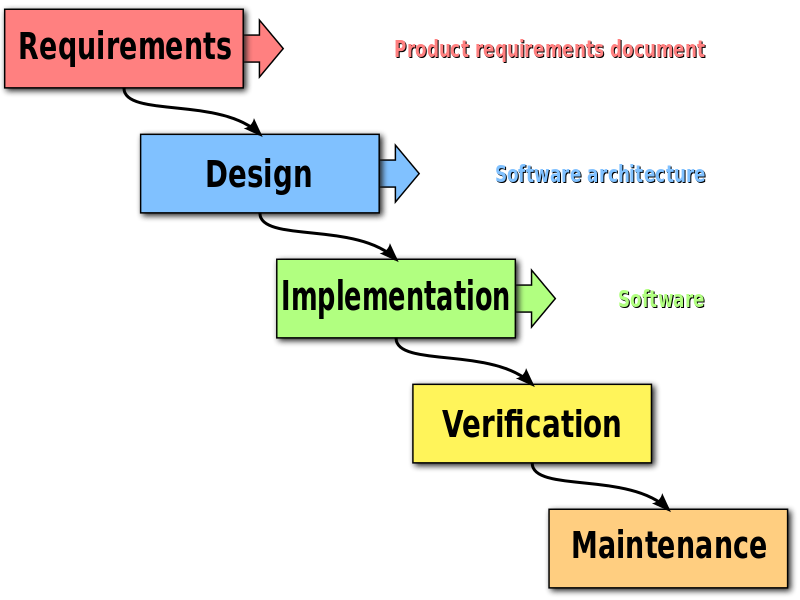
\includegraphics[width=0.8\textwidth]{images/Waterfall-model.png}
\caption{Unmodified Waterfall Model \cite{waterfallModel}}
\label{fig:Waterfall_model}
\end{figure}

\newpage
\subsubsection{Scrum}
The scrum development method is an agile approach to development. It is an iterative process consisting of several cycles or iterations. Each cycle, called a \emph{Sprint}, lasts a set length of time, typically one week to one month (7-30 days).

Within each of these cycles, most of the phases of a sequential method are covered. A sprint starts with a sprint planning session, where tasks to be completed in the sprint are planned and prioritized. The majority of the sprint consists of completing these tasks, which usually are parts of the solution that then needs to be integrated into the complete product. The sprint should result in a functioning prototype, presented to the customer at the end of the sprint to receive feedback for the next sprint, and concludes with a sprint review meeting.

The following figure depicts the typical flow in agile methods.

\begin{figure}[H]
\centering
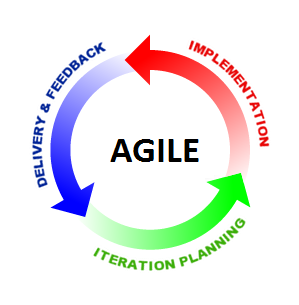
\includegraphics[width=0.8\textwidth]{images/agile-methods.png}
\caption{Agile Methods \cite{agileModel}}
\label{fig:agile_model}
\end{figure}

\subsubsection{Our choice}
Each of the proposed methods have their own advantages and disadvantages, that make each of the methods respectively a better or worse fit for our project than the other.

While the different methods have various advantageous features, not all of these are applicable to our particular project, and others are negligible.

Below we have highlighted the most important advantages and disadvantages of each method, while discussing whether or not the particular point is relevant to our project, leading to a conclusion and our choice of method. \\ \\
\emph{Waterfall} \\ \\
The following points are advantages of using the Waterfall method for projects, both in general and for ours specifically.
	\begin{itemize}
		\item Waterfall is suitable for small projects because they are manageable to fully plan up front. This fits our project description.
		\item It is easier to get every involved party on the same page with a thorough plan, such as provided through the Waterfall method's early phases. This is beneficial to any project, but even more so in one such as ours, where the team consists of students who may have other projects in other courses running in parallel with this.
	\end{itemize}
These next points are generally advantages of the Waterfall method, but are mostly not applicable for our project for various reasons.
	\begin{itemize}
		\item Waterfall is a good method if you know everything about the project beforehand, or are able to acquire the required information and the full project specification before the implementation phase. Due to the course schedule and the relatively limited time frame of our project, we felt we needed to start implementation earlier than a long planning and requirements phase would allow.
		\item Sequential methods require little under-way feedback. This gives them the edge over agile methods when access to the customer is restricted but specifications are expected to remain the same. While the specifications for our project were expected to remain unchanged, our goal was to include the customer in the process.
		\item The method supplies strong documentation as the first phases are focused entirely on creating these documents. However, while the course relies heavily on documentation, the customer had no use for most of this documentation, making this point less important for our project.
	\end{itemize}
Lastly we have the biggest disadvantage of following a sequential method, which applies to any project doing so.
	\begin{itemize}
		\item Sequential methods don't handle change to the requirements particularly well, making this approach risky in the case of the customer wishing to modify the requirements during the implementation phase.
	\end{itemize}

\emph{Scrum} \\

Advantages of agile methods such as scrum include the following:
	\begin{itemize}
		\item Agile methods support rapid production of prototypes to present to the customer. This allows for easier correction of misunderstandings, because they become apparent earlier in the process through the functioning prototypes.
		\item The method utilizes stand-up meetings, a scrum master, and optionally (and preferably) a scrum board. These things do carry overhead, but provide both the team and customer with frequent feedback, making the benefit much greater than the disadvantage of the overhead.
		
		\begin{figure}[H]
		\centering
		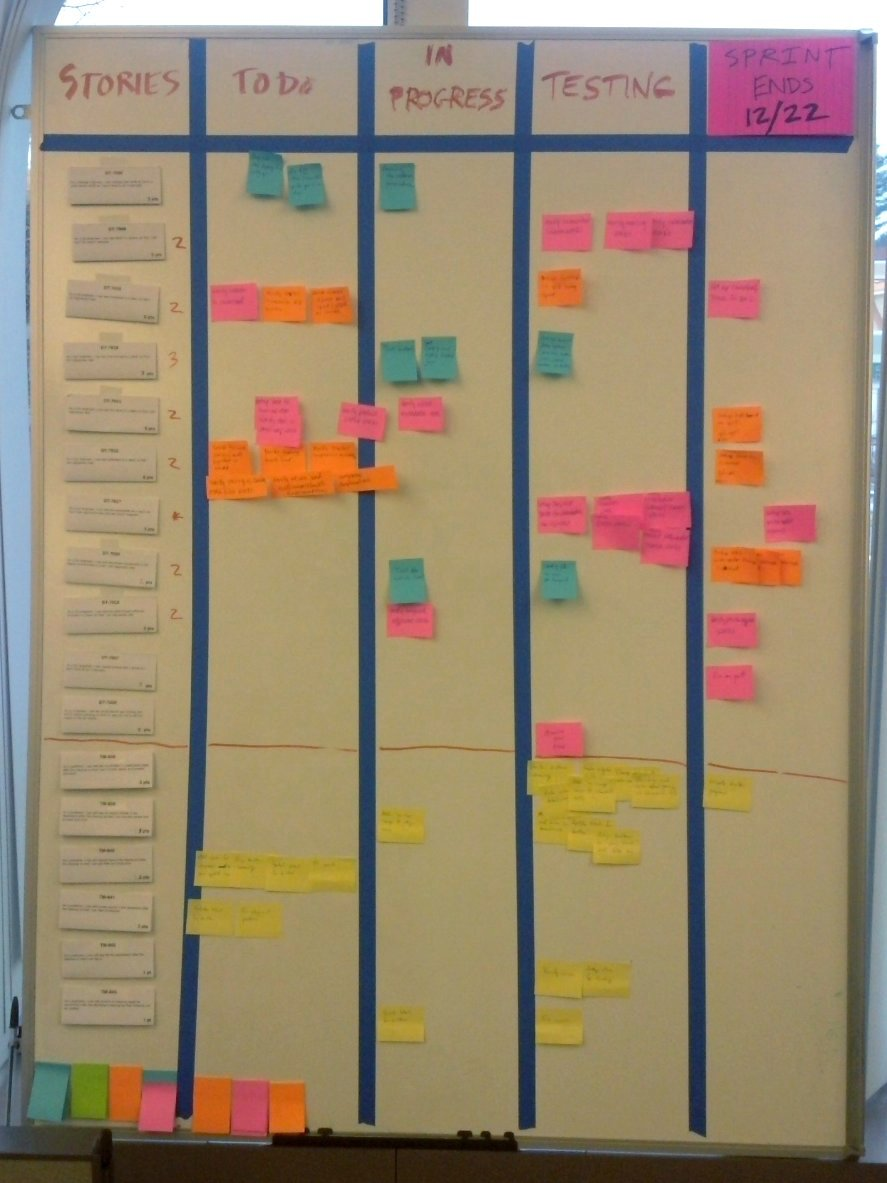
\includegraphics[width=0.8\textwidth]{images/Scrum_task_board.jpg}
		\caption{Example Scrum Board \cite{scrumBoard}}
		\label{fig:scrum_board}
		\end{figure}
		
		\item The approach is highly supported by online tools - e.g. Trello for the scrum board - that let both parties (the team and the customer) stay up-to-date on the planning and prioritization of tasks during implementation.
	\end{itemize}
While the next point generally is an advantage of agile development over a sequential process, it does contain some risks for a small project such as ours, as explained below.
	\begin{itemize}
		\item Agile methods handle change to requirements very well, due to the high level of underway involvement of the customer. The risk of weighting this point when deciding on an approach is the possibility that there simply will not be many changes, making this point irrelevant. Because we expected there to be necessary changes to the requirements and specification during the implementation, we decided this was important for our project.
	\end{itemize}
There is one major disadvantage - or rather, risk - of choosing an agile approach.
	\begin{itemize}
		\item Agile methods rely on team members - or at least the project manager - having experience with the full development process, assuming the entire project is to be completed in agile fashion.		
	\end{itemize}
There is another important point when using an agile method, which can be the deciding factor for some projects.
	\begin{itemize}
		\item Iterative approaches are heavily reliant on easy access to the customer for continuous feedback and extraction of requirements. This is okay for our project, as our customer is readily available through both e-mail and phone.
	\end{itemize}

From our analysis of the two methods, we concluded that neither were a perfect fit for every part of our project. We felt that our inexperience with projects such as this one made it too difficult to complete the entire project through an agile process, but we felt too unsure about the scope of the project to plan everything ahead and do a straight sequential process. We did, however, wish to plan an outline for the project, create a general architectural overview and gather the most important requirements before we started implementation.

This led us to a decision of employing the waterfall method, or at least something similar, for the complete process, with a relatively long period of planning before starting implementation.

The customer suggested using an agile approach for implementation because it is the same as they use. Using the same method as the customer might be beneficial to the project, as it improves communication and work flow. We decided to complete the implementation phase as an agile process, divided into two-week sprints, each consisting of a sprint planning meeting, then several days of implementation, with semi-daily stand-up meetings, and ending in a sprint review meeting and a functioning prototype.

\subsection{In Practice}
While we planned to utilize a combination of the two methods as described above, we ended up with something a little different in practice.
\newpage

\subsection{Frameworks}
\subsubsection{Software Development Model}
\subsubsection{Programming languages, Communication Protocols and File Formats}
\subsubsection{Web Api}
\subsubsection{Server}
To run the web api framework there's IIS express that comes with visual studio 2012. The express version is meant to be used for developing purposes, when deploying the product a full version of IIS should be used.
\subsubsection{Database}
We had a lot of problems with the database, the customer said he'd put up a database server for us to use. However this turned out to be difficult to achieve due to the security/confidentiality issues on their server. We had to try to set up the database server ourself on our local machine, this proved to be rather difficult due to Microsoft tools not giving enough information, and thereby not installing the necessary tools. Some of us communicated via SMS and phone services.

The customer uses an MSSQL server and they provided an 11 GiB .bak file which we could use to restore the database.
\documentclass[12pt, a4paper]{article} 
 
\usepackage[utf8]{inputenc}
 
 
\usepackage{geometry} % to change the page dimensions
\geometry{a4paper} % or letterpaper (US) or a5paper or....
 
\usepackage{graphicx} % support the \includegraphics command and options
 
\usepackage{booktabs} % for much better looking tables
\usepackage{array} % for better arrays (eg matrices) in maths
\usepackage{paralist} % very flexible & customisable lists (eg. enumerate/itemize, etc.)
\usepackage{verbatim} % adds environment for commenting out blocks of text & for better verbatim
\usepackage{subfig} % make it possible to include more than one captioned figure/table in a single float
% These packages are all incorporated in the memoir class to one degree or another...
 
 
 
\usepackage{amsmath, amssymb}% for mathematical symbols
\usepackage[colorlinks=true,linkcolor=black, urlcolor=blue]{hyperref} % for hyperreferences with black color
%\usepackage[T1]{fontenc} % Uncomment for norwegian document
%\usepackage[norsk]{babel} %
 
%%% HEADERS & FOOTERS
\usepackage{fancyhdr} % This should be set AFTER setting up the page geometry
\pagestyle{fancy} % options: empty , plain , fancy
\renewcommand{\headrulewidth}{0pt} % customise the layout...
\lhead{}\chead{}\rhead{}
\lfoot{}\cfoot{\thepage}\rfoot{}
 
%%% SECTION TITLE APPEARANCE
\usepackage{sectsty}
\allsectionsfont{\sffamily\mdseries\upshape} % (See the fntguide.pdf for font help)
% (This matches ConTeXt defaults)
 
%%% ToC (table of contents) APPEARANCE
\usepackage[nottoc,notlof,notlot]{tocbibind} % Put the bibliography in the ToC
\usepackage[titles,subfigure]{tocloft} % Alter the style of the Table of Contents
\renewcommand{\cftsecfont}{\rmfamily\mdseries\upshape}
\renewcommand{\cftsecpagefont}{\rmfamily\mdseries\upshape} % No bold!

\begin{document}

\section{Technology}

\subsection{Windows 7, 8}
Microsoft Windows 7 and - 8 are operating systems by the Microsoft Corporation. They logically provide good support for .NET developments, seeing as .NET targets the Windows platform and is made by Microsoft. Visual Studio is made for Windows, and was our main IDE, so all team members had access to PCs with Windows installed.

\subsection{Ubuntu Linux}
This OS is perhaps the most widely used distribution of Linux, developed by Canonical Ltd. It provides good support for many development tools, except of course Windows development. However we did find support for using it for some Windows development.
This operating system was used by one team-member on a laptop, when working on-site at NTNU. For coding, Mono with MonoDevelop was used, while other tasks were mostly unaffected. The operating system provides good support for other parts of the process, such as Git and \LaTeX.

\subsection{Mac OSX}
%TODO

\subsection{Visual Studio 2012}
Visual Studio is Microsofts IDE for development for their platforms. This is the main IDE we developed the framework on, seeing as it has very good integration with C\# and .NET platforms, which we were required to use.

\subsection{.NET and Mono}
We were required to use ASP .NET MVC for our framework. ASP .NET MVC is a framework for web applications which enables the use of the Model View Controller (MVC) pattern. It is part of Microsofts .NET Framework suite, which is the preferred way of interactiong with Windows systems and OSes.

Mono is the open source-, cross-platform version of the .NET suite, which we used when not developing on Windows machines. It is available both for Windows, OS X, most Linux Distributions, Android, and various other operating systems.

\subsection{MonoDevelop}
This is an open source IDE for development with Mono, available for OS X and most Linux distributions. This was the IDE used when not developing on Windows machines.

\subsection{LaTeX}
We quickly chose \LaTeX \ for our typesetting. It being the de-facto standard for academic typesetting, with good support for both code snippets, tables, references and bibliography.

Most of our group also had at least some experience using it, and some were quite experienced, which made the choice easier.

\subsection{Git}
For our version control and source repository, we chose Git. This because we had most experience with it, and found it easy to set up via GitHub (where we all had accounts already). It also has the advantage of being distributed, so we could avoid a single point of failure, and having a staging area where one can selectively commit files according to whether they're ready or not, instead of risking accidental changes which might break something.

Both the source code and the entirety of the report source files were stored on GitHub, since both would be catastrophical to lose, and were quite important to have under version control in case we needed to track problematic changes.

\subsection{Trello}
To support our agile process and sprints, we used Trello for planning and control of workflow. It is an online Kanban Board tool, where we can create work packages and issues, while tracking who does what, and tracking backlog, finished modules, and work in progress.

\subsection{Web API}
%TODO

\subsection{Dropbox}
\href{http://www.dropbox.com}{Dropbox} is a syncing service that let you choose a local folder on your machine that will be synced to the cloud. Dropbox lets you share folders and files inside a shared Dropbox folder.

We used Dropbox for sharing and synchronizing internal documents that usually were only useful for a limited time, but might be referenced later.

\subsection{Google Drive}
\href{https://drive.google.com/}{Google Drive} is Google's office pack. The difference between Drive and other office solutions (like Microsoft Office , OpenOffice/LibreOffice) is that Drive exist in the cloud and lets the user simultaneously work on a document.

Google Drive was used for simultaneous collaboration on documents, where the content was up for discussion, or it was advantageous to see what the others where writing.

\end{document}

\subsection{Templates}
We have created the following templates for documents used in the process:

\begin{itemize}

\item Foo
\item Bar

\end{itemize}
We have established several standards for the project, as seen in the rest of this section.

\subsection{Documents}
For internal documents we have established the naming standard:

MM\_DD\_<Description>\_<Version if applicable>
\\
This is to ensure documents are properly sorted, and that they are easily identifiable.



\subsection{Coding}
We will be using C\# as a programming language, and will consequently be following the C\# coding standards, as outlined by Microsoft <cite http://msdn.microsoft.com/en-us/library/vstudio/ff926074.aspx here>.
\\\\
The guidelines are summarized in the following section.\\

\subsubsection{Documentation}
All public classes, methods, and preferably properties/fields shall be documented with comments which will enable generation of documentation. Example:
\begin{lstlisting}
/// <summary>
/// This is a summary of what the class contains and its intended function
/// </summary>
/// <author>Author Name</author>
public class ExampleClass
{
	/// <summary>
	/// This summary tells what the method does, any side-effects, and how/why to use it.
	/// It should NOT say how the method does what it does, unless this is absolutely neccessary.
	/// </summary>
	/// <param name="intName">int</praram>
	/// <param name="stringName">String</praram>
	/// <returns>String</returns>
	/// <author>Author Name</author>
	public abstract String ExampleMethod(int intName, String stringName);
}
\end{lstlisting}

\subsubsection{Naming and variables}
Use CamelCase for classes, method names and properties.
Example:
\begin{lstlisting}
public class ExampleClass
{
	public abstract void ExampleMethod(int intName, String stringName);
	
	private int ExampleProperty { get; set; }
}
\end{lstlisting}

Variables shall be named after the lowerUpper scheme, where the first word is in lowercase, and any others starts with an uppercase letter.
Example:\\
\begin{lstlisting}
int exampleVariable = 1;
int stringExample = "This is an example";
\end{lstlisting}

\subsubsection{Comments and layout}
Blocks shall start and end with curly brackets on their own line.

Comments shall have a space between the double slashes and the actual comment. Continuation lines shall be indented. All comments shall start with a capital letter, and end with a period.

There shall be only one statement per line. The same goes for declarations. Parantheses shall be used to separate clauses in expressions, to ease understanding.

\begin{lstlisting}
// This is a single line comment
void Foo()
{
	// The following is correct:
	int x;
	int y;
	
	// The following is incorrect:
	int x,y;
	
	// This is a multi line comment, with more text this is line two of a multi line comment

	
	if(true)
	{
		StatementOne();
		StatementTwo();
		
		if ((var1 && var2) || (var3 && var4))
		{
			Bar();
		}
	}
}
\end{lstlisting}

\subsubsection{Variables, types, and declaration}
Implicitly typed local variables can be used when the right hand side clearly indicates type, or it's not important.

Use in-line instantiation with constructors when possible, instead of instantiation and assignment.

Short strings shall be appended with the use of the + operator. Longer ones in loops shall use StringBuilder.\\

Example:
\begin{lstlisting}
// Apparent use of string. Use of var ok:
var name = "SampleString";

// Type inconsequential:
foreach(var v in collection)
{
	//Type-independent method:
	handleVar(v);
}

// Array instantiation with constructor:
int[] numbers = { 1, 2, 3, 4 };

//Use of var requires explicit instantiation
var numbers2 = new int[] { 1, 2, 3, 4 };

//Avoid this if you could have used the above:
int[] numbers3 = new int[4];
numbers3[0] = 1;
numbers3[1] = 2;
// Etc.

//Short string example
string simpleString = "This is our " + var1 + "test-string." + var2 + "something."

//String builder example
string longString = "LongLongLong";
var longBuilder = new StringBuilder();
for(int i = 0; i < 1000; i++)
{
	longBuilder.Append(longString);
}

\end{lstlisting}


\subsubsection{Try-catch, exceptions and using}
Exception handling shall be done by try-catch statements.
Code shall not unexpectedly throw exceptions; only when something unrecoverable has happened.

In the case of a try-finally statement, a using statement shall be used instead, if the only function of
the finally-block is disposing/closing of the used object.
\\
\begin{lstlisting}
Socket socket = new Socket();
try
{
	socket.SomeMethod();
}
finally
{
	socket.Close();
}
// Can be replaced by:
using (Socket socket = new Socket();)
{
	socket.SomeMethod();
}
\end{lstlisting}

\subsection{Static Members}
Static members shall always be called by class name, and never accessed in a derived class when defined in a base class.

\subsubsection{Clean Coding}
We have also endeavoured to follow the ten Clean Coding principles, as outlined by one extra pixel's post. \cite{cleanCoding}
The ten principles are as following:
\begin{enumerate}

\item Revise your logic before coding
\item Clearly expose the structure of the page
\item Use the correct indentation
\item Write explanatory comments
\item Avoid abusing comments
\item Avoid extremely large functions
\item Use naming standards of functions and variables
\item Treat changes with caution
\item Avoid indiscriminate mixing of coding languages
\item Summarize your imports

\end{enumerate}

\subsection{APIs}
\subsubsection{ASP .NET Web API}
One of the agreed upon requirements for the project was that we conform to ASP .NET Web API. This to make it easier to interact with our framework from other systems (both existing and future ones). An introduction to using this API can be found at \href{http://www.asp.net/web-api}{http://www.asp.net/web-api} or \href{http://msdn.microsoft.com/en-us/library/hh833994(v=vs.108).aspx}{http://msdn.microsoft.com/en-us/library/hh833994(v=vs.108).aspx}.

\subsection{Summary}